% !TEX option = --shell-escape
\documentclass[a4paper,12pt]{scrartcl}
\usepackage[x11names,dvipsnames,svgnames]{xcolor}
\usepackage[a4paper,top=2.5cm,bottom=2.5cm,left=2cm,right=2cm]{geometry}
\usepackage{cmap,microtype}
\usepackage[utf8]{inputenc}
\usepackage[T1]{fontenc}
\usepackage{doc}
%\usepackage[scale=.87]{tgheros}
%\usepackage{tgtermes}
%\usepackage[lite]{mtpro2}
\usepackage{libertine}
\renewcommand\ttdefault{txtt}
\usepackage{dirtree}

\usepackage{relsize}
\usepackage[smallcaps]{glossaries}
%\loadglsentries{acronymlist}
\newacronym{UKM}{ukm}{Universiti Kebangsaan Malaysia}

\usepackage{graphicx,tabularx,booktabs,wasysym,multicol,textcomp}
\usepackage[os=win]{menukeys}
\usetikzlibrary{matrix}
\usepackage{enumitem}
%\setlength\pltopsep{6pt}
% \usepackage{listings}
% \lstset{language=[LaTeX]TeX,columns=fullflexible,
% basicstyle=\ttfamily\small,texcsstyle=*\bfseries\color{NavyBlue},
% commentstyle=\itshape\color{PaleVioletRed4},
% emphstyle=\bfseries\color{BrickRed},
% frame=single,framesep=6pt,
% framexleftmargin=6pt,framexrightmargin=6pt,
% xleftmargin=12pt,xrightmargin=12pt,
% breaklines=true,breakatwhitespace=true}
\usepackage{minted}
\setminted{breaklines,frame=single,framesep=6pt,breaksymbol={}}
% \usemintedstyle{borland}

\usepackage{hyperref,cleveref}
\usepackage{apacite}
\bibliographystyle{apacite}

\newcommand{\GayaUKM}{\textsf{GayaUKM}}

\title{Guide on Using GayaUKM}
\subtitle{version 1.4}
%\author{Zambri, Rasidi, Asyraf, Wajdi, Lian, Khamisah, Kamal\\\texttt{\smaller zambri\string@eng.ukm.my,liantze\string@gmail.com}}
\author{\normalsize
%\begin{tabular}{l l}
\begin{tikzpicture}
\matrix[matrix of nodes,ampersand replacement=\&,right delimiter={\} \texttt{@gmail.com}}]{
\textbf{\textsc{Lim} Lian Tze (\texttt{liantze})} \& Zambri Harun (\texttt{zambriharun}) \\
Rasidi Rasani (\texttt{rasidi.rasani}) \& Asyraf Zulkifley (\texttt{asyraf.zulkifley})\\
Wajdi Sadik (\texttt{wajdisadik}) \& Khamisah Jafar (\texttt{kjafar61})\\
};
\end{tikzpicture}
%\end{tabular}
}

\publishers{\large Pusat Pengurusan Siswazah \\
Universiti Kebangsaan Malaysia}

% \date{\large November 28 2013}
% \date{\large November 4, 2017}
\date{\large May 19, 2019}
\begin{document}
\maketitle

\GayaUKM{} is a \LaTeX\ class for authoring theses that fulfill formatting specifications required by \gls{UKM}, Malaysia. Why \LaTeX? %It seems that publishers of reputable journals have given attentions to manuscripts or articles using \LaTeX. UKM feels that a guideline on thesis using \LaTeX\ is necessary to promote general writing using the latter.
Many reputable journals prefer manuscripts to be prepared and submitted using \LaTeX\ to ensure consistent adherance to formatting requirements. \gls{UKM} therefore feels that a \LaTeX\ class and guidelines for authoring theses is necessary to promote general document authoring using \LaTeX.

The sample files \texttt{thesis-english.tex} and \texttt{tesis-bahasa.tex} are made available as the main guides in the package. It is recommended that authors develop their own arrangement when writing up their own theses. Authors can rename the files, however `\texttt{thesis-english.tex}' (i.e.~the English version) will be referred to throughout this guide.

The authors of the guideline feel that this is only the first steps to using \LaTeX. There is a wide range of areas in which theses authors can improve or develop further upon. There are many packages available to fulfill various needs, e.g.~plotting or equations, in different faculties. Theses authors are welcome to use relevant packages for their own needs; however they should not use packages that could alter the general arrangements required by the main thesis formatting specifications.

Some understandings of using higher languages are recommended but not necessary. For first time \LaTeX\ users, authors are recommended to get `head starts' from more experienced colleagues, especially if this is the authors' first experience using \LaTeX.

\clearpage
\tableofcontents
\section{Before You Start}
\subsection{Printing from Acrobat Reader}
This is such an important point that I've decided to make it the \emph{first} section:

In the \menu{Print...} dialog, remember to
\begin{itemize}[noitemsep]
\item set the \textbf{paper size} to \textbf{A4};
\item set \textbf{page scaling} to \textbf{None} or \textbf{Actual size} or \textbf{100\%},
\end{itemize}
otherwise the page margins and visual font sizes would be incorrect!

\subsection{Files}

Here's a quick list of the files required when writing your thesis with the \GayaUKM{} class. Easiest way to go about things is to put all the files in the same directory. %(See \Cref{sec:howto} for more details.)
%
\begin{itemize}[noitemsep]
\item \texttt{\bfseries GayaUKM.cls}, the \LaTeX\ class file implementing the \gls{UKM} thesis formatting requirements.
\item \texttt{\bfseries GayaUKM.bst}, the \BibTeX\ bibliogaphy (English) style file.
\item \texttt{\bfseries GayaUKM-ms.bst}, the \BibTeX\ bibliography (Bahasa Melayu) style file.
\item \texttt{\bfseries thesis-english.tex}, a sample English thesis \texttt{.tex} file using \texttt{GayaUKM.cls}.

\item \texttt{\bfseries tesis-bahasa.tex}, a sample Bahasa Melayu thesis \texttt{.tex} file using \texttt{GayaUKM.cls}.

\item \texttt{\bfseries refs.bib}, a sample bibliography database file. %(See \Cref{sec:bibliography}).
%\item A \texttt{.tex} file containing your glossary. (See \Cref{sec:glossary}).

\item Various \texttt{*.tex} files forming the contents of the sample theses.
\end{itemize}

{\large Things should work if you put all these files in the same directory and start editing your own thesis.}

For the more technically advanced users: If you want to install \GayaUKM{} `properly' in your own TEXMF tree, see the next subsection. (This is not compulsory to start using \GayaUKM{}.)


\subsection{File Installation (Optional: For Technically Advanced Users)}

\begin{enumerate}
\item \menu{Windows Start>MikTeX>Maintenance (Admin)>Settings (Admin)}
\item Click on \menu{Roots} tab.
\item Create a new directory on your system, e.g.~\directory{C:/llt-texmf}.
\item \keys{Add...} a user \texttt{\$TEXMF} tree, and specify \directory{C:/llt-texmf} as the new tree. Click \keys{OK}.
\begin{center}
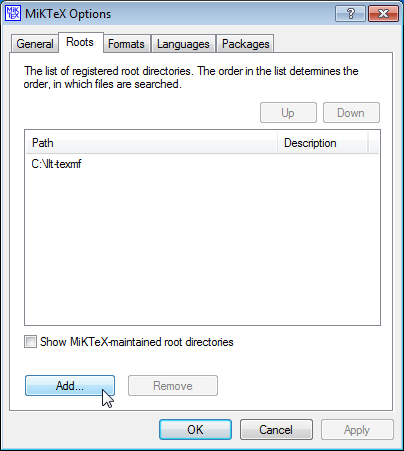
\includegraphics[width=.455\linewidth]{user-texmf}
\end{center}

\item Copy \texttt{GayaUKM.cls}, \texttt{GayaUKM.bst} and \texttt{GayaUKM-ms.bst} to your user tree as follows:%, e.g.\\\path{C:/llt-texmf/tex/latex/GayaUKM/GayaUKM.cls}.

\begin{minipage}{.5\textwidth}
\dirtree{%
.1 C:\textbackslash.
.2 llt-texmf.
.3 tex.
.4 latex.
.5 GayaUKM.
.6 GayaUKM.cls.
.3 bibtex.
.4 bst.
.5 GayaUKM.
.6 GayaUKM.bst.
.6 GayaUKM-ms.bst.
}
\end{minipage}

\item Click on \menu{General} tab, \keys{Refresh FNDB}:
\begin{center}
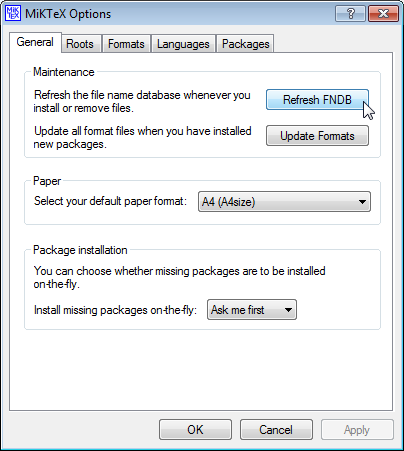
\includegraphics[width=.455\linewidth]{refresh-fndb}
\end{center}
\item Your \LaTeX\ system can now use \texttt{GayaUKM.cls} from any path.
\item (Mac users: Copy the \texttt{.cls} file to \path{~/Library/texmf/tex/latex/GayaUKM/}, and \texttt{.bst} files to \path{~/Library/texmf/bibtex/bst/GayaUKM/}. You're good to go.)
\item (\textsmaller{GNU}/Linux users: Copy the \texttt{.cls} file to \path{~/texmf/tex/latex/GayaUKM/}, and \texttt{.bst} files to \path{~/texmf/bibtex/bst/GayaUKM/}. Then run {\ttfamily texhash} as \emph{normal user}.)
\end{enumerate}

\section{Compiling \texttt{thesis-english.tex} (and similarly \texttt{tesis-bahasa.tex})}
The processing tools should be run on \texttt{thesis-english.tex} (and similarly \texttt{tesis-bahasa.tex}) in the following sequence:
\begin{enumerate}[noitemsep]
\item \texttt{pdflatex}
\item \texttt{bibtex}
\item \texttt{pdflatex}
\item \texttt{pdflatex}
\end{enumerate}


\section{Writing Your Thesis with \LaTeX}\label{sec:latex:howto}

\subsection{Activation}\label{sec:activation}
To `activate' the class, make sure your main document file (e.g.\ \texttt{thesis-english.tex} or \texttt{tesis-bahasa.tex}) starts off with \mintinline{latex}{\documentclass[language]{GayaUKM}}:

\medskip%\enlargethispage{\baselineskip}

\begin{minted}{latex}
\documentclass[english,nohyphen]{GayaUKM}   %% For English
\usepackage{graphicx}
\usepackage{... other packages you need}
\end{minted}

OR

\begin{minted}{latex}
\documentclass[bahasa,nohyphen]{GayaUKM}    %% untuk Bahasa Melayu
\usepackage{graphicx}
\usepackage{... other packages you need}
\end{minted}

\medskip

This will set up the page margins, paragraph spacing, indents, page numbers, font face and size, language settings, chapter and section headings, citation and bibliography format, amongst other things. Use the \texttt{nohyphen} option to disable hyphenation. However please do \emph{not} import the \texttt{subcaption} or \texttt{subfigure} packages as they will interfere with \GayaUKM{}'s caption settings. See section~\ref{sec:floats} to see how to use subcaptions (for sub-figures and sub-tables) in \GayaUKM{}.

\subsection{Author Information}\label{sec:author:info}
You need to provide some author information in the preamble. Example lines from \texttt{thesis-english.tex}:

\medskip

\begin{minted}{latex}
\title{<Your Thesis Title>}
\author{<Your Name>}
\authorid{<P00000 ID No.>}
\faculty{<Your Faculty>}
\submissiondate{2 October 2013}
\submissionyear{2013}
\degreetype{Doctor of Philosophy}
\campus{Bangi}
\end{minted}

\medskip

These information are needed to generate the preliminary pages. Sometimes you may be asked by the Graduate Office to format your title into a reverse pyramid, so will need to insert manual line breaks into the title: you can do this with \mintinline{latex}{\protect\\}. For example:
\begin{minted}{latex}
\title{<Your Thesis Title, Manually Break\protect\\the Lines into a Nice Reverse\protect\\Pyramid if Necessary>}
\end{minted}

\subsection{Preliminary Pages}
Once in the main document body, \mintinline{latex}{\frontmatter} sets up the, well, front matter. This include setting the page numbers to lower-case Roman numerals. \mintinline{latex}{\maketitle}  generates the cover and title page. \mintinline{latex}{\declaration} can generate the declaration.

\begin{minted}{latex}
\begin{document}
\maketitle

\frontmatter
\declaration
\end{minted}

Since the cover page and title page uses different font sizes, you may want to use different manual line-breaking schemes for these two pages, so that the reverse pyramids look better on both pages. In this case you can first generate \emph{only} the cover page with \mintinline{latex}{\makecoverpage}, re-issue the \mintinline{latex}{\title} with different manual line break positions, and then generate \emph{only} the titlepage with \mintinline{latex}{\maketitlepage}, like this:

\begin{minted}{latex}
\title{<Your Thesis Title, Manually Break\protect\\the Lines into a Nice Reverse\protect\\Pyramid if Necessary>}
....
\begin{document}
\makecoverpage

\title{<Your Thesis Title, Manually Break the Lines into a Nice\protect\\ Reverse Pyramid if Necessary>}
\maketitlepage

\frontmatter
...
\end{minted}

The English and Malay abstracts, and the acknowledgements, are typeset with the \texttt{enAbstract}, \texttt{msAbstract}, \texttt{acknowledgements} environments:

\begin{minted}{latex}
\begin{enAbstract}
This is the English abstract. ...
\end{ebAbstract}

% The Malay translation of your title needs to be given here
\begin{msAbstract}[<Terjemahan Tajuk Tesis dalam Bahasa Melayu>]
Inilah abstrak dalam Bahasa Melayu.

\begin{acknowledgements}
This is the acknowledgements. ...
\end{acknowledgements}
\end{latex}

Note that the translated title of your thesis needs to be given for the translated abstract. (In the sample files, the English abstract, Malay abstract, acknowledgements, as well as each separate chapter, are each placed in separate files and \mintinline{\input} into the main thesis file.)

\bigskip

This is followed by the content lists:

\begin{minted}{latex}
\tableofcontents
\listoftables
\listoffigures
\end{minted}

\subsection{List of Symbols, etc}
These can be prepared using tables. An example is given in \texttt{symbols.tex}, to typeset a List of Symbols:

\begin{minted}{latex}
\chapter{List of Symbols}
\begin{center}
\doublespacing
\begin{tabular}{l@{\hspace{3em}}p{.6\textwidth}}
$b, c$ & constants\\
$C_f$ & local friction coefficient\\
\end{tabular}
\end{center}
\end{minted}

Use a \href{https://texblog.org/2011/05/15/multi-page-tables-using-longtable/}{\texttt{longtable}} or \texttt{supertabular} instead if your list is longer than a page: normal \texttt{tabular}s cannot automatically break across pages.

\subsection{Main Chapters}
Start the main text of your thesis with \mintinline{latex}{\mainmatter}, followed by the usual chapters and sections:

\begin{minted}{latex}
\mainmatter
\chapter{Introduction}
...
\section{...}
\end{minted}

You may want to use \mintinline{latex}{\input} to better organise your chapter files as shown in the sample files.


\subsection{Tables and Figures}
\label{sec:floats}

All tables and figures may be created as usual practice in \LaTeX. You may use extra packages like \texttt{booktabs}, \texttt{tabularx}, \texttt{longtable}, \texttt{tabu}, etc.~as needed.

\emph{Updated in v1.2:} Sources of tables and figures are acknowledged using the \mintinline{latex}{\source} command \emph{below} the \mintinline{latex}{\caption}:

\begin{minted}{latex}
\begin{figure}[hbt!]\centering
  \includegraphics[width=8cm]{architecture.jpg}
  \caption{Architectural design of system}
  \source{Original Source of Diagram}
\end{figure}
\end{minted}


To add captions for sub-figures and sub-tables, use the \mintinline{latex}{\subcaption} command:

\begin{minted}{latex}
 \begin{figure}[hbt!]\centering
 \includegraphics[width=.9\textwidth]{graph1}    % subfigure a
 \subcaption{Results using ABC}

 \includegraphics[width=.9\textwidth]{graph2}    % subfigure b
 \subcaption{Results using XYZ}

 \caption{Performance of ABC and XYZ}   % the MAIN caption of this figure
 \end{figure}
\end{minted}

\subsection{Citations and Bibliography}
Specify your Bib\TeX\ database file (e.g.~\texttt{refs.bib}) with

\begin{minted}{latex}
\bibliography{refs}
\end{minted}

You may use \texttt{natbib} citation commands:

\begin{center}
\begin{tabular}{ll}
\toprule
\bfseries\centering\arraybackslash Command & \bfseries\centering\arraybackslash Output\\
\midrule
\mintinline{latex}{\cite{Edwards:2013}} & (Edwards 2013)\\
\mintinline{latex}{\citep{Edwards:2013}} & (Edwards 2013)\\
\mintinline{latex}{\citet{Edwards:2013}} & Edwards (2013)\\
\mintinline{latex}{\cite[p.~28]{Edwards:2013}} & (Edwards 2013, p.~28)\\
\mintinline{latex}{\citeauthor{Edwards:2013}} & Edwards\\
\mintinline{latex}{\citeyear{Edwards:2013}} & 2013\\
\mintinline{latex}{\citeyearpar{Edwards:2013}} & (2013)\\
\bottomrule
\end{tabular}
\end{center}

\subsection{Appendices}
If you have any appendices, you can add them thus:
\begin{minted}{latex}
\appendix
\chapter{Sample Code}
...
\end{minted}

You may want to use \mintinline{latex}{\input} to better organise your appendix files as shown in the sample files.


\end{document}
